\chapter{Technical Foundation}
\label{cha:technical_foundation}

This chapter provides the technical foundations that are used for the solution that has been developed by this thesis.
These overviews do not go into detail about how they are used in this thesis but rather aim to provide
a foundation for the reader which is required by the following chapters.
Section \ref{sec:tech_containerization} explains the concept of containerization as well as the concepts of Kubernetes and Helm.
Section \ref{sec:tech_monitoring_systems} explains the concept of monitoring systems and their components.
Additionally, this section provides the foundations for the tools used by the monitoring solution that was developed for this thesis.

\section{Containerization}
\label{sec:tech_containerization}

\begin{figure}[tb]
	\centering
	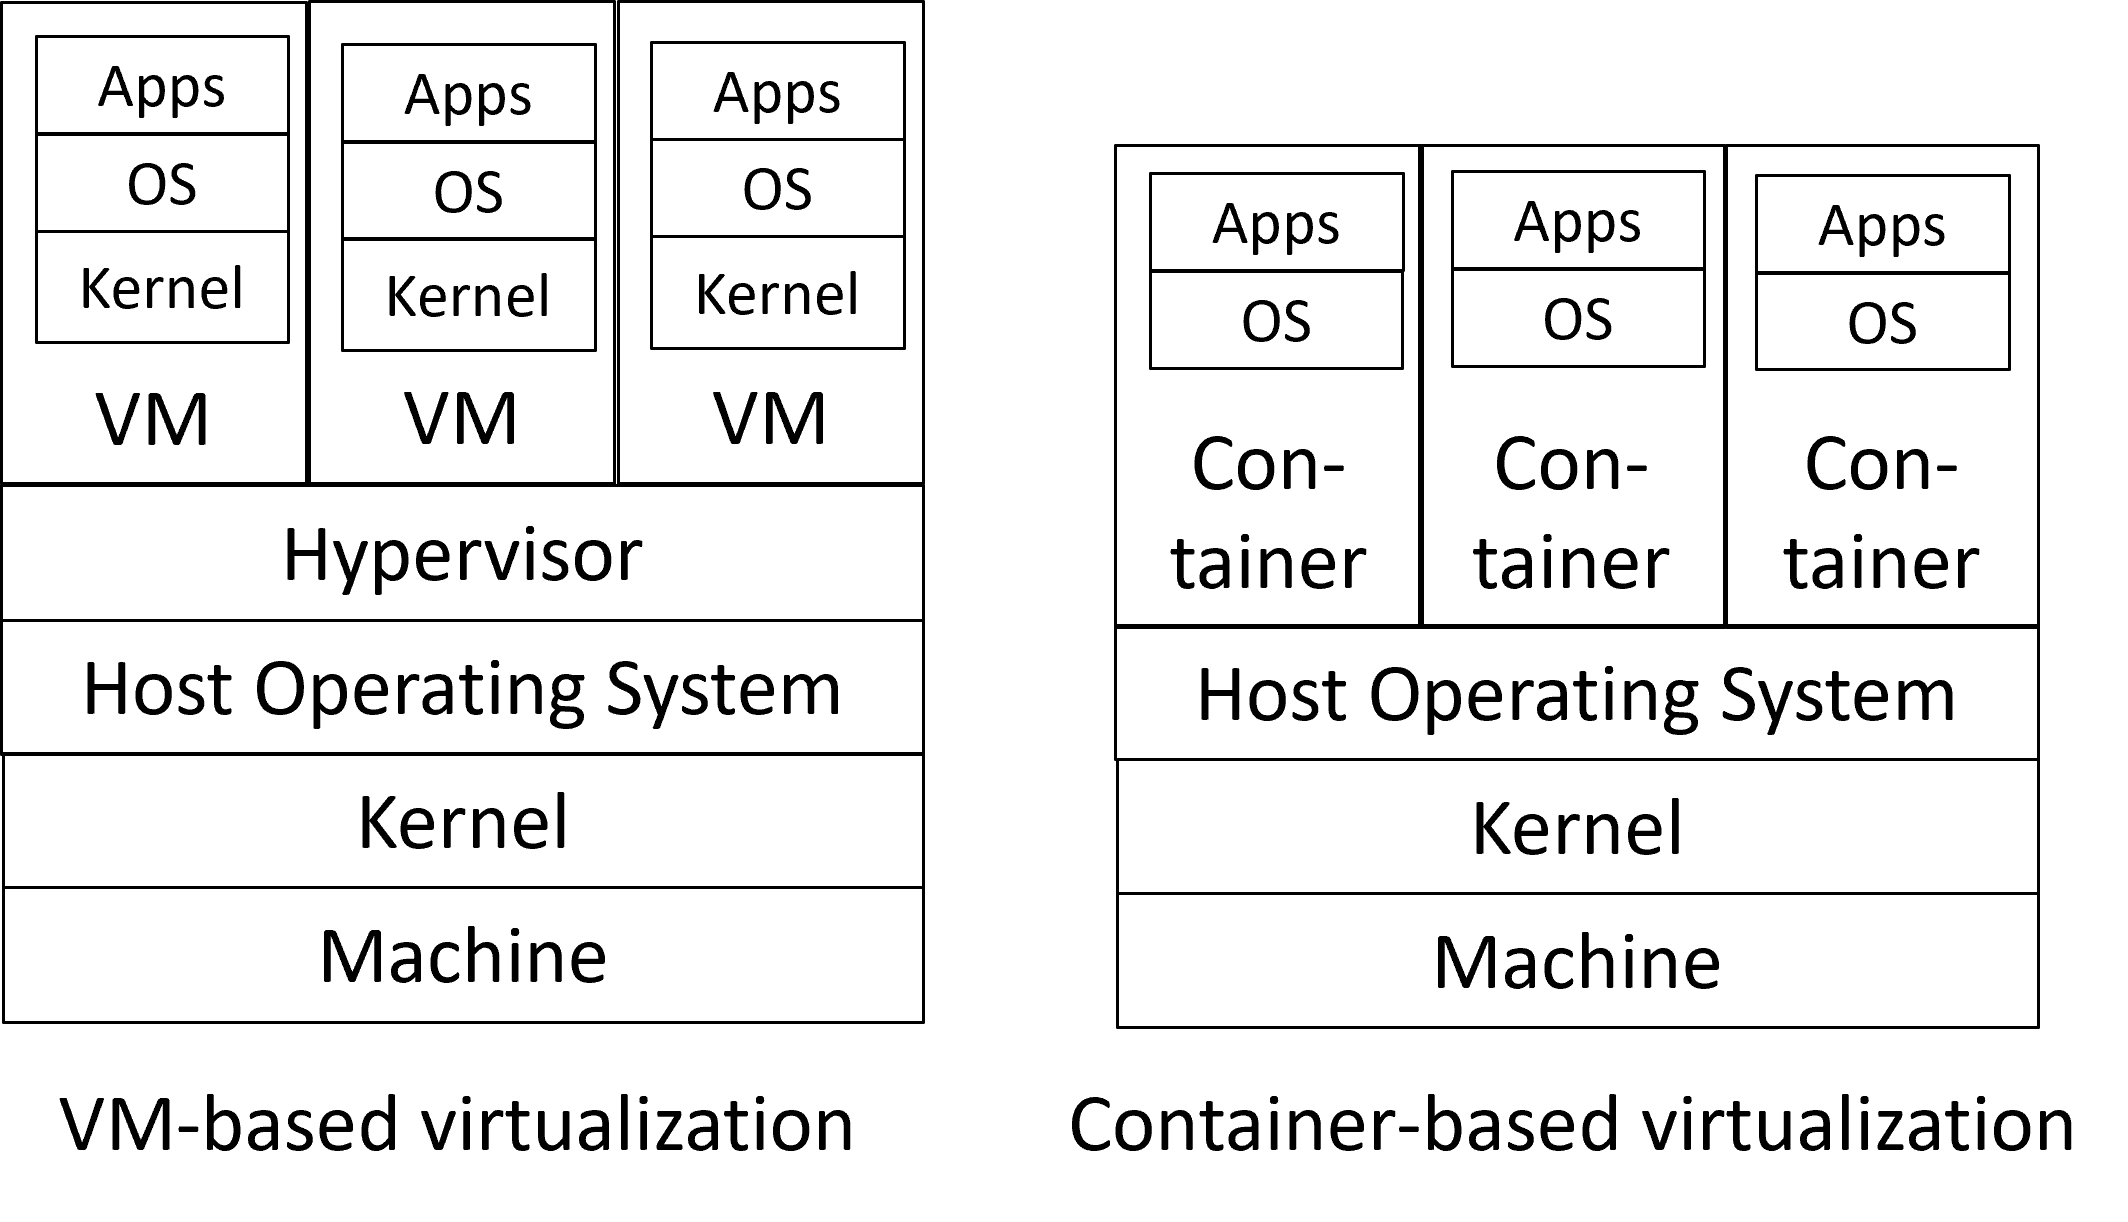
\includegraphics[width=0.7\textwidth]{figures/vm_container_virtualization.png}
	\caption{VM vs. Container-Based Virtualization \cite{CM-W-CON}}
	\label{fig:vm_container_virtualization}
\end{figure}

Containerization is one of two possibilities to virtualize IT infrastructure.
The first possibility is virtualization through virtual machines.
The second possibility is containerization. The difference between virtual machines
and containerization is how they operate. This is visualized in Figure \ref{fig:vm_container_virtualization}.
Virtual machines run in a separate operating system complete with a separate kernel on top of the host machine's
operating system. The two operating systems are controlled by a Hypervisor that manages the scheduling of both
operating systems. Contrarily, containers run directly in the host machine's operating system
in separate process spaces to restrict their access to the host machine.
While virtual machines provide more security, containers are more lightweight in their overhead
and easier to set up. Because of this, containerization is the most common approach to virtualizing
IT infrastructure in cloud environments.

\subsection*{Kubernetes}

Kubernetes \cite{KUB-DOCS} is a tool that provides container orchestration and deployment
for clusters of servers. Container orchestration consists of scheduling containers and workloads
onto different servers depending on their available resources and managing state changes like updates
for containers. 
A cluster in Kubernetes consists of one or more nodes that represent a server that hosts a container runtime.
Kubernetes schedules containers and other resources automatically onto different nodes
depending on factors like the current workload of a node.
The smallest unit in Kubernetes' scheduling is a Pod. A Pod is a grouping of one or more containers.
Kubernetes also provides additional resources for networking, configuration, access control, and storage.
Some of the other resources available in Kubernetes are described below.

Eleven resources in Kubernetes are important for this thesis.
These resources are listed below with a brief description.
\begin{itemize}
	\item \textbf{Deployment} \\
	A Deployment describes the desired state for a Pod.
	The state of a Pod includes properties like the number of replicas,
	the version of a container's image, or a container's open ports.
	Kubernetes manages the incremental change of a Deployment to reach its desired state.
	\item \textbf{Service} \\
	A Service provides logical endpoints within a cluster.
	Each endpoint on a service is mapped to a port on a specified Pod.
	\item \textbf{Ingress} \\
	An Ingress provides access to the cluster from external networks via, for example, HTTP.
	An Ingress maps endpoints on the cluster to ports on services within the cluster.
	Ingresses can also provide additional functionality like load-balancing.
	\item \textbf{ConfigMap} \\
	A ConfigMap is a resource that can store data as key-value pairs.
	The values of a ConfigMap can be simple YAML properties or file-like.
	\item \textbf{Secret} \\
	A Secret is a type of ConfigMap that is meant to hold confidential data.
	\item \textbf{PersistentVolume (PV)} \\
	A PV provides access to a storage medium. PVs can be statically or dynamically
	provisioned.
	\item \textbf{PersistentVolumeClaim (PVC)} \\
	A PVC requests access to a PV on behalf of an application.
	Each PVC contains information like the requested storage size and access mode (read/write).
	\item \textbf{ServiceAccount} \\
	A ServiceAccount is an account for accessing a cluster. ServiceAccounts are meant
	to be used by resources running within a cluster. Each ServiceAccount has a set of
	permissions for what it is allowed to access in the cluster.
	\item \textbf{ClusterRole} \\
	A ClusterRole combines a set of permissions for a ServiceAccount into a named role.
	\item \textbf{ClusterRoleBinding} \\
	A ClusterRoleBinding binds a ClusterRole to a ServiceAccount which gives
	the ServiceAccount the permissions defined in the ClusterRole.
	\item \textbf{CustomResourceDefinition (CRD)} \\
	A CRD allows the definition of additional custom resources for Kubernetes.
\end{itemize}

\subsection*{Helm}

Helm \cite{HEL-DOCS} provides templating for Kubernetes resources.
Natively, Kubernetes only supports static resource definitions that can only
be configured by manually changing the resource's definition. Additionally,
Kubernetes does not provide any support to always set related properties
in resource definitions to the same values. Helm solves this issue
by providing Helm Charts that bundle multiple resource definitions
with a configuration file. The values from the configuration file
can be used to template the resource definitions. Helm manages the templating and
installation of the resources within a Chart into a Kubernetes cluster. This allows
for Charts of applications to be shared via registries that can then be configured to
each user's needs. Helm uses the Golang programming language
for its templating engine. In addition to templating simple values from a configuration file
into a resource's definition, the usage of Golang allows control flow structures and
some pre-defined function calls to be made. With this, the complete structure of a resource's
definition can be changed. This enables, for example, features of a Chart to be turned on or off
depending on the configuration of the Chart.
An example of how Helm works can be seen in \autoref{lis:helmExample}.
Values from the configuration file can be accessed by putting the property's name in double curly braces and prefixing it with .Values,
as can be seen in line 2 of the listing.

\begin{figure}[tb]
\begin{lstlisting}[caption = {Helm Templating Example}, label = {lis:helmExample}, style = kit-cm, language=yaml]
# Template file
name: app-{{ .Values.name }}

# values.yaml
name: example

# Rendered Kubernetes file
name: app-example
\end{lstlisting}
\end{figure}

\section{Monitoring Systems}
\label{sec:tech_monitoring_systems}

A complete monitoring system requires three main parts: Data sources, data sinks, and the ability
to analyze/visualize the collected data.
The collected data can be split into three different types
according to the three pillars of observability: Metrics, Logs, and Traces.
Because this work only focuses on metrics, logs and traces will be ignored for this explanation of monitoring systems.

Data sources are the origin of the collected metrics and can be split into two different types
based on how they acquire metrics. The first type is data sources that perform manual instrumentation.
This means that the application source code is amended by code that collects metrics and emits them.
Manual instrumentation is useful for application-specific metrics, like for example, how often a user
uses a certain feature in the application.
The second type is data sources that perform automatic instrumentation.
These data sources collect metrics from applications or the environment without changing any source code.
In contrast to manual instrumentation, automatic instrumentation is limited to collecting
common metrics that are provided by an application and its environment like CPU or memory usage.

Data sinks store the metrics that were collected by the data sources.
It is important to note that some data sinks specialize in which type of data they store
to increase efficiency. The last part is the analysis and visualization of the collected metrics.

Optionally, a monitoring system might employ additional components such as data transformers or collectors.
Data transformers can be used to transform data into different formats, enrich it with additional information
or aggregate it.
Data collectors can be used to buffer metrics that were sent by data sources before they are stored in a data sink,
which decreases the load on the data sink.